\section{Introduction}

Numerous astronomical observations suggest the existence of a substance that permeates the universe and appears to only interact significantly with ordinary matter via gravity. 
Attempts to directly observe it have been unsuccessful, but this mysterious ``dark matter'' is estimated to make up over a quarter of the total mass-energy in the universe. 
The possibility that dark matter interacts with ordinary matter by other means besides gravitation remains open, implying dark matter may be produced directly by the LHC. 
If produced, dark matter particles are practically invisible to the detector and manifest as missing energy in the event. 
This document describes a search for dark matter produced in association with $\ttbar$ in the dilepton channel with data collected by the CMS detector in 2016 of $\PP$ collisions at $13\:\TeV$.

The simplest and most relevant model for dark matter production with $\ttbar$ proposes a spin-$0$ interaction between dark matter (DM) and Standard Model (SM) particles. 
If the new physics associated with DM satisfies minimal flavour violation, where the couplings between the mediator and the SM particles are Yukawa-type, then heavy flavour (top quark) production is favoured. 
At leading order, the process is gluon-induced and a $\ttbar$ pair is produced with a pair of DM fermions (Fig.~\ref{fig:ttdm_diagram}). 
%The DM fermions can be Dirac or Majorana with the difference being a factor of two in the cross section; they are taken to be Dirac fermions in the signal samples used in this analysis.

\begin{figure}
\centering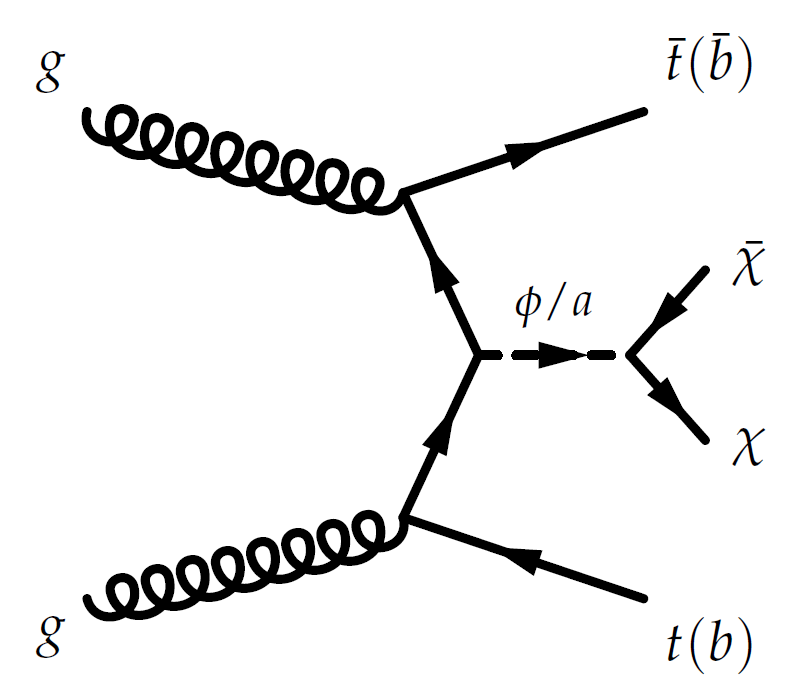
\includegraphics[width=8cm]{figures/ttbarDM.png}
\caption{Leading order diagram in simplified model for $\ttbar+$DM production.}
\label{fig:ttdm_diagram}
\end{figure}

  We use events with two opposite-sign isolated leptons, and two jets with at least one b-tagged jet to perform the search. The stransverse
  mass variable \mtll~\cite{Lester:1999tx} is used to separate the dark matter signal from the Standard Model background, which consists primarily of \ttbar pairs decaying to the dilepton channel.
  The stransverse mass is a generalization of the transverse mass \mt to a system of pair produced particles that decay semi-invisibly. 
  In the case of $W$ boson production, \mt is formed from the transverse momentum of a high \pt lepton (from the $W$ decay) and the missing transverse momentum (\met) in the event, 
  which is assumed to come from the corresponding neutrino. The definition of \mt in the limit where the masses of the daughter particles can be neglected is given by

  \begin{equation}
    \label{eq:mt}
    \mt = \sqrt{2 E_\ell \met \left[1 - \cos(\Delta\phi)\right]}
  \end{equation}

  The transverse mass has the property that if the lepton and the \met both come from the decay of a
  single particle with mass $m$, then $\mt \leq m$. In order to generalize to a system with two particles
  of the same mass, each decaying semi-invisibly, we have to decompose the measured \met into
  a sum of two missing transverse momentum vectors according to %as in Equation~\ref{eq:METsplit}:
 
  \begin{equation}
    \label{eq:METsplit}
    \mathbf{p}_T^{miss} = \mathbf{p}_{T1}^{miss} + \mathbf{p}_{T2}^{miss}.
  \end{equation}

  We may then pair each missing transverse momentum vector with the visible products of the
  decay in order to form \mt for each leg of the pair production. However, since the correct division of the \met into two components is not known, 
  a useful method is to minimize the maximum of the two transverse masses formed under all possible combinations satisfying Equation~\ref{eq:METsplit}. 
  That is, we explore the parameter space of all possible hypothetical neutrino momenta
  that satisfy Equation \ref{eq:METsplit} and for each point in this parameter space we calculate \mt for each half
  of the event and report the maximum of the two. We take the \mtll value for the event to be the
  minimum of the larger \mt value for each such point. This can be represented as %by the expression  for \mtll given in Equation~\ref{eq:mt2ll}:

  \begin{equation}
    \label{eq:mt2ll}
    M_{T2}^2(ll) = \min_{\mathbf{p}_{T1}^{miss} + \mathbf{p}_{T2}^{miss} = \mathbf{p}_T^{miss}} \left( \max \left[ \mt^2(\mathbf{p}_T^{\ell1},\mathbf{p}_{T1}^{miss}) , \mt^2(\mathbf{p}_T^{\ell2},\mathbf{p}_{T2}^{miss}) \right] \right)
  \end{equation}

  It can be shown~\cite{Lester:1999tx} that this definition of \mtll has the same convenient property as the transverse mass: 
  it must be less than the mass of the pair-produced semi-invisibly decaying particle.
  In the case of \ttbar+DM searches in the dilepton channel, the primary challenge comes from separating SM \ttbar 
  production from the signal, since the composition of the final states is identical except
  for invisible particles. In dileptonic \ttbar events the final state is

  \begin{equation*}
    pp \to t + \bar{t} + X \to bW^+ + \bar{b}W^- + X \to b\ell\bar{\nu}_\ell + \bar{b}\bar{\ell}\nu_\ell + X.  
  \end{equation*}

  Assuming that the contribution of the other products $X$ to the \met is not large, the assumptions
  made in the definition of \mtll hold for the lepton-\met system and its value has an upper
  bound at the $W$ mass. On the other hand, dark matter production according to Fig.~\ref{fig:ttdm_diagram}
  provides two extra invisible particles.
  Hence, partitioning of  \met into two components no longer needs to respect an upper bound at the W mass.

  Similarly, one is also able to construct two other variants on the \mtll variable, which take into account the $b$-jets and are expected to have an upper bound at the top mass:

  \begin{align}
    \label{eq:mt2bb}
    M_{T2}^2(bb)   &= \min_{\mathbf{p}_{T1}^{miss} + \mathbf{p}_{T2}^{miss} = \mathbf{p}_T^{miss}} \left( \max_{b \in b_1,b_2} \left[ \mt^2(\mathbf{p}_T^{b},\mathbf{p}_{T1}^{miss}) \right] \right) \\
    M_{T2}^2(lblb) &= \min_{\mathbf{p}_{T1}^{miss} + \mathbf{p}_{T2}^{miss} = \mathbf{p}_T^{miss}} \left( \max_{b \in b_1,b_2, \ell \in \ell_1, \ell_2} \left[ \mt^2(\mathbf{p}_T^{b} + \mathbf{p}_T^{\ell}, \mathbf{p}_{T1}^{miss}) \right] \right)
  \end{align}
  There are two choices how to pair the two leptons  and the two b-jets in the case of \mtlblb. This ambiguity is resolved by minimizing the maximum invariant mass of the two lepton-jet pairs.

  The analysis strategy described in the note uses this property of \mtll, \mtbb and \mtlblb in order to construct
  signal regions, with $\mtll > M_W$, that should have a small
  contamination from dileptonic top decays stemming from the Standard Model.
